% !TEX encoding = UTF-8 Unicode
% !TEX program = pdflatex
% !TEX spellcheck = en_US


% In order to correctly compile this document,
% execute the following commands:
% 1. pdflatex
% 2. pdflatex
% 3. pdflatex



\documentclass[amsthm,ebook]{saparticle}

% IF YOU USE PDFLATEX
\usepackage[utf8x]{inputenc}
% if you write in english and in greek
\usepackage{ucs}
\usepackage[greek,english]{babel}
\languageattribute{greek}{polutoniko}

% IF YOU USE XELATEX
%\usepackage{polyglossia}
% if you write in italian
%\setmainlanguage{italian}
% If you want put some ancient greek:
%\setotherlanguage[variant=polytonic]{greek}
%\newfontfamily{\greekfont}[Ligatures=TeX]{Palatino Linotype}

% dummy text (remove in a normal thesis)
% remove if not necessary
\usepackage{siunitx}
%Natbib for bibliography management
\usepackage[authoryear]{natbib}
% custom commands
\newcommand{\bs}{\textbackslash}

%%%%%%%%
%TITLE:%
%%%%%%%%
\title{I.Sicily. An EpiDoc corpus for ancient Sicily}
\author[OXF]{Jonathan Prag\corref{first}}
\author[opensky]{James Chartrand}
\author[OXF]{James Cummings}
\address[OXF]{University of Oxford}
\address[opensky]{OpenSky Solutions}
\cortext[first]{Corresponding author. Email: jonathan.prag@merton.ox.ac.uk}
\date{2015-11-18}
\begin{document}

\maketitle
\begin{abstract}
This paper introduces the EpiDoc corpus of inscriptions on stone for ancient Sicily, I.Sicily. The project is one of the
first attempts to generate a substantial regional corpus in EpiDoc. The project is confronting a number of challenges
that may be of wider interest to the digital epigraphy community, including those of unique identifiers, linked data,
museum collections, mapping, and data conversion and integration, and these are briefly outlined in the paper.
\end{abstract}
\keywords{Sicily, Epigraphy, Epidoc, Greek, Latin, Pleiades, multilingualism}




\section{Introduction: What is I.Sicily}


I.Sicily is an online, open access, digital corpus of the inscriptions on stone from ancient Sicily.\footnote{ The
corpus will be mounted at \url{www.csad.ox.ac.uk/sicily/isicily}, but is presently on a development server. A public face is
currently maintained via a blog at \url{http://isicily.wordpress.com/}, as well as on Facebook at \url{www.facebook.com/ISicily}
and on Twitter via \url{I.Sicily@Sicilyepigraphy}.} The corpus aims to include all texts inscribed on stone, in any language,
between approximately the seventh century BC and the seventh century AD. The corpus currently contains records for over
2,500 texts, and when complete is likely to contain c.4,000. The corpus is built upon a conversion from a legacy
dataset of metadata in MS Access to EpiDoc TEI XML.\footnote{\url{http://sourceforge.net/p/epidoc/wiki/Home/} [accessed
26.09.2015].} The XML records are held in an eXist database for xQuery access, and additionally indexed for full-text
search using SOLR/Lucene. The corpus and related information (museum list, bibliography) are published as Linked Data,
and are manipulated through a RESTful API. The records are queried and viewed through a web interface built with
AngularJS and jQuery javascript components. Mapping is provided in the browser by the Google Maps API, and ZPR (Zoom,
Pan, Rotate) image-viewing is provided by the IIIP image server and the OpenSeadragon javascript library.
%IIIP or IIIF ? I believe this is a typo

At the time of writing (September 2015), the main conversion routine is being refined and the epigraphic texts are being
collated for incorporation into the records. An ancillary database of museum collections in Sicily has been constructed
and bibliography is held in a Zotero library. Extensive search facilities will be provided, including map-based and
bibliographic searching. Individual inscriptions and individual museums will both be provided with URIs, as will
personal names and individuals; places will be referenced using Pleiades; epigraphic types, materials, and supports
using the EAGLE vocabularies.

\section{The motivations for and origins of I.Sicily}


The existing epigraphic landscape in Sicily is extremely diverse in two primary regards: on the one hand, the island has
a very mixed cultural and linguistic make-up, meaning that the epigraphic material is itself extremely varied, with
extensive use throughout antiquity of both Greek and Latin, as well as Oscan, Punic, Sikel, and Hebrew;\footnote{
Recent overview of much of the linguistic tradition in \citet{tribulato_language_2012}; and of the epigraphic material in \citet{gulletta_sicilia_1999}.} on the other hand, the publication of this material has a very uneven record and despite an excellent
pre-twentieth century tradition, the existing copora are far from complete and the ability of key journals such as SEG
or AE to keep pace with local publication has been limited.\footnote{ For an overview of the corpora tradition up to
the twentieth century, see \citet{de_vido_corpora_1999}.} A limited number of museum-based corpora have been published in recent
decades (for Catania, Palermo, Messina, and Termini Imerese, as well as the material from Lipari), but this has not
greatly improved the overall situation.

The combination of these two factors already means that locating, identifying, or working with a Sicilian inscription,
or its publication record, is extremely challenging for anyone without extensive experience of the material. The
situation is compounded by the universal and familiar challenges of the recording and accessibility of archaeological
collections, whether held in museums, in archaeological stores, or elsewhere, and the lack of consistency in the
publication of \ new material.

As noted in the introduction, some of the impetus for I.Sicily comes from a desire to exploit a substantial legacy
dataset in MS Access. This consists of a single table originally constructed in MS Access 2000, and maintained
erratically from the year 2000 onwards. The original purpose of this table was to gather data to assess the `epigraphic
habit' of ancient Sicily, and consequently the texts themselves were not the primary focus. However, the extent to
which the dataset facilitated further study made increasingly clear its potential value for the study of Sicilian
epigraphy.\footnote{ The principal results were published in \citet{prag_epigraphy_2002}, revised in \citet[159-188]{prag_sicily_2004}; cf. \citet{prag_nouveau_2003}, \citet{prag_ciceronian_2007}, \citet{prag_sicilia_2008}, \citet{prag_sicilia_2010}.}

In its final form the table holds data across 39 different fields, for 2575 records. 17 of these fields detail
publication history (corpora references and other bibliography); the other fields record information on the language,
date, provenance, current location, epigraphic type, form and material of the inscriptions, together with a free-text
field recording further information about the inscription and fields to record any autopsy undertaken. Almost all of
this data is derived from existing publications.

The conversion from the original MS Access dataset was developed through a pipeline of known conversions going from MS
Access to CSV to TEI P5 XML. The XSLT transformation of the table of data from TEI P5 XML to EpiDoc XML is the point in
the process where further up-conversions of the data were made. These include the creation of the hierarchical EpiDoc
XML as well as normalisation of dating and bibliographic records. This conversion is not meant to be repeated as the
dataset, once converted to EpiDoc XML, will be edited in the I.Sicily website. While the conversion preserves the data
from the MS Access dataset, it restructures and where possible improves or normalises it.

By virtue of the fact that I.Sicily begins from such rich metadata, to which texts, images, and further data will be
added over time, and because this is in turn being supplemented by an on-going programme of autopsy, the form and
content of I.Sicily is intended to be more akin to that of a true corpus than simply a text-database, seeking to
combine a full record of past publication and study with a fully revised edition, and potential for multiple
individuals to contribute to a process of on-going revision (see Fig.~\ref{fig:1} for a draft edition of one inscription (AE
1962.314 = I.Sicily 820)).




\section{The aims of I.Sicily}


We outline briefly five areas in which I.Sicily aims to develop, facilitate and improve the study of epigraphic material
from ancient Sicily.




\subsection{Multilingualism}


Sicily is traditionally described as a `melting pot', the `crossroads of the Mediterranean'. The negative consequences
of the separation of epigraphic material according to linguistic traditions have recently been highlighted and directly
confronted by the Corpus Inscriptionum Iudaeae/Palaestinae (CIIP), edited by H. Cotton et al.\footnote{ Original notice
in \citet{cotton_corpus_1999}; presentation in \citet{cotton_corpus_2010}.} I.Sicily sets out to follow in that mould, since the
different linguistic traditions of Sicily not only exist side-by-side but interact constantly throughout the island’s
history, and no study of the epigraphic material can afford to ignore contemporary and parallel material in the other
languages.\footnote{ See e.g. \citet{manganaro_greco_1993}, \citet{prag_epigraphy_2002}, \citet{salmeri_i_2004}, \citet{korhonen_language_2011}, \citet{tribulato_language_2012}.} The situation
created by basic technologies such as Unicode and EpiDoc XML mean that there is now no reason not to be language
agnostic in the inclusion of material (the point may be obvious, but the tendency towards language-specific corpora is
still marked). The opportunities and possibilities offered by these technologies are considerable, even at the most
basic level, since, for example, searching can be made language specific or language neutral. One obvious area where
Sicilian studies are currently hampered by this partitioning is in the study of onomastics. The Lexicon of Greek
Personal Names records most instances of Greek names for the island, but Sicily is no less rich in non-Greek names
(Latin and others), and at present there is no onomasticon for the island.\footnote{ \url{www.lgpn.ox.ac.uk/} [accessed
26.09.2015].} Simply by the marking-up and indexing of all names in the island’s inscriptions, I.Sicily will generate a
powerful tool for future study. Although I.Sicily in its first phase is not undertaking morphological or syntactical
mark-up, the encoding of all these text in XML constitutes the necessary first stage in such a development, and we see
this as a highly desirable future project, and the possibilities for the field of historical linguistics are
considerable. The incorporation of a full range of metadata on the epigraphic support, geographical location,
chronology, etc. will likewise allow detailed analysis of cultural patterns and their relationship to language-use over
time.\footnote{ See Prag 2002 for a first effort in this direction.}




\subsection{Identification and Bibliography}


Sicily presents a particularly extreme version of the common problem of identifying a text and its publication record.
No existing corpus in either Greek or Latin comes close to full coverage (CIL X and IG XIV are the largest individual
traditional corpora for the region, but both are over 125 years old and cover less than 30\% of the material now
known).\footnote{\citet{_inscriptiones_1883}; \citet{kaibel_inscriptiones_1890}.} Existing online databases improve on this situation, but the results
obtainable are of very varied value. The most comprehensive, in terms of the range of data recorded, is EDR (with which
I.Sicily is collaborating), which currently reports 1,906 records for `Sicilia'; but this reduces to 833 when limited
to texts on stone (`lapis' or `marmor'); contrast I.Sicily, with 2,563 records at the time of writing.\footnote{
\url{www.edr-edr.it/} [accessed 26.09.2015]} Clauss Slaby reports 4,374 records for `Sicilia' (including Christian
inscriptions, excluding `sigilla impressa'), but the return is inclusive of all kinds of epigraphic material, without
indication or discrimination, contains some duplication, is much harder to reconcile to existing records, and records
only text.\footnote{ \url{www.manfredclauss.de/} [accessed 26.09.2015].} The PHI database of Greek inscriptions has a rich
record of published Greek texts, but is text only and limited in outputs.\footnote{
\url{http://noapplet.epigraphy.packhum.org/regions/1156} [accessed 26.09.2015].} SEG references are available for 733
inscriptions on stone and AE references for 328 (data taken from the I.Sicily database and based upon comprehensive
manual trawls of SEG and AE).

One major aim of I.Sicily, therefore, is to generate unique identifiers for each inscription - the I.Sicily number, in
the form ISic 1234. These will be maintained as URIs, of the form:

\url{http://csad.ox.ac.uk/sicily/inscription/ISic1234}

I.Sicily is well placed to do this since its initial dataset is primarily a bibliographic concordance of the lapidary
inscriptions of Sicily. One of the associated outputs of the project will therefore be an online bibliography for
Sicilian epigraphy, and an online Zotero library has already been created with over 700 records which are referenced in
the EpiDoc files.\footnote{\url{www.zotero.org/isicily} (private at the time of writing, but to be made public when the main
site is launched) [accessed 26.09.2015].} A locally cached version of the bibliography will be presented at the
I.Sicily site to facilitate detailed bibliographic searching (including the identification of inscriptions by
publication) and to allow the generation of customised concordances.

A further element of bibliographic information which I.Sicily will include is the cross-referencing and linking to
online editions of major antiquarian corpora of Sicilian inscriptions. A growing number of these are already available
in digital format and several are already mounted in the Arachne archive, making direct page-citation
possible.\footnote{ E.g. Castelli 1784, at \url{http://arachne.uni-koeln.de/books/Castelli1784} [accessed 26.09.2015].}

The richness of I.Sicily’s records in this area mean that I.Sicily is currently collaborating with both Trismegistos and
IDES (`Integrating Digital Epigraphies').\footnote{\url{www.trismegistos.org/} [accessed 26.09.2015] and \url{http://ides.io/}
[accessed 26.09.2105].} The former aims to generate TM numbers for all the Sicilian material (which I.Sicily will
include); the latter is to assist IDES in the refining of links between, e.g., PHI and SEG records, and to improve
I.Sicily’s own recording of PHI numbers.




\subsection{Identification and Collections}


The traditional focus of epigraphic study upon the text, rather than the epigraphic support, means that epigraphic
publication in the past has frequently been relatively limited in the information which it has recorded about the
object on which the inscription is inscribed. This is a familiar complaint, and one which I.Sicily will address
wherever possible through full object description and a rich photographic record. However, a corollary of this general
problem is a very low level of information regarding current location and in particular the infrequent recording of
museum inventory numbers or similar information. This situation is inevitably exacerbated by the substantial (and very
positive) reorganisation and redevelopment of museum collections in Sicily recent decades – including a significant
increase in the number of museums and public collections.

I.Sicily is making use of the TEI {\textless}msIdentifer{\textgreater} element, with its associated sub-elements in
order to record details of institutional collections and inventory numbers wherever possible.\footnote{\url{www.tei-c.org/release/doc/tei-p5-doc/en/html/ref-msIdentifier.html} [accessed 26.09.2015].} In order to maximise the
value of this, we have adopted two further courses of action. In the first place, as part of the larger ambition of
undertaking autopsy of every stone contained within the corpus, we are working in close collaboration with museums on
the island to improve our records of individual museum holdings. Where possible we aim to include associated archival
information, such as copies of inventory records. This work currently includes a major sub-project to catalogue the
epigraphic collection of the Museo Archeologico Regionale Paolo Orsi at Siracusa, and we are also currently working
with collections at Adrano, Halaesa (Tusa, ME), and Catania.\footnote{ We gratefully acknowledge the ongoing support of
dott.ssa G. Lamagna and dott.ssa A.M. Manenti at Siracusa, as well as previous directors of the Museo Archeologico at
Siracusa, dott.ssa C. Ciurcina and dott.ssa B. Basile; of dott.ssa A. Merendino at Adrano; of dott.ssa G. Tigano and
dott. R. Burgio at Messina; and of dott.ssa M.G. Branciforte at Catania.} It is hoped that this work will be of
considerable value to the museums themselves, since access to the I.Sicily records should facilitate the curation,
display and accessibility of the inscriptions (see below also on translations), and we welcome future collaboration
with other museums on the island.

Secondly, in collaboration with Dr Michael Metcalfe, I.Sicily has developed a database of Sicilian archaeological
collections (130 at the time of writing). This database is mounted online alongside the epigraphic corpus, in a
searchable format, including map-based searching. In order to facilitate the generation of linked data, the individual
museum records will be maintained with URIs, of the form:

\url{http://csad.ox.ac.uk/sicily/museum/SicMus123}

The linking of the epigraphic and museum databases will enable the searching and reporting of inscriptions by museum
collection as well as the easy locating of the appropriate collection.




\subsection{Location, location, location}


I.Sicily is actively generating rich geo-data for the individual inscriptions, both for the original findspot/provenance
and the current location (whether museum-based, on-site, or elsewhere), and we aim to provide map-based searching for
inscriptions, as well as text-based searching by ancient and modern place-names. In addition to full listing wherever
possible of both ancient and modern place names for epigraphic provenance, we are working to provide detailed location
information for each find-spot and the inscription’s current location, through a combination of library and map-based
research and the use of autopsy and GIS recording. At present geo-data is being recorded in two forms, both through the
use of explicit geographical locations in the form of longitude and latitude records in decimal degree form (using
{\textless}geo{\textgreater} elements), and through the use of Pleiades URI references wherever possible.\footnote{
\url{http://pleiades.stoa.org/} [accessed 26.09.2015].} We are committed to the long-term use of Pleiades as our primary
reference for ancient places, and to that end we aim to update and improve the Pleiades data for Sicilian locations, in
particular name data and sub-locations, in conjunction with the editing of the I.Sicily records.\footnote{ See e.g.
\citet{wilson_places:_2015}. Valeria Vitale (KCL) is currently undertaking a significant programme of data improvement in
Pleiades on behalf of I.Sicily; we are grateful to Tom Elliott and Jeffrey Becker for their support.}




\subsection{Searching}


In order to support the aims outlined above, I.Sicily has taken a different approach to search and browse. Although
standard form-based search with paged results, like that of Google, makes sense for very large result sets, the
comparatively small number of records in I.Sicily (thousands versus the estimated 30 trillion web pages indexed in
Google) lends itself to a more direct and interactive approach - a spreadsheet/grid model (similar to Microsoft Excel)
that runs directly in the browser. Although it is tempting to repeat the standard web-form model, following the
argument that that’s what users expect, the spreadsheet approach will be much easier to use, narrowing quickly and
accurately to more easily interpreted results. Further, any subset of the spreadsheet, generated from interactive
filtering, can, with a single button push, be exported to CSV (comma separated values) for use outside I.Sicily. The
spreadsheet interacts particularly well with maps: all findspots or museums in a filtered subset of the grid can be
simultaneously shown on the map (see Fig.~\ref{fig:2}). The spreadsheet model also provides a very quick and intuitive (since so
many people are familiar with spreadsheets) means for editing records (in this case, inscriptions and museums) online.
This web-based spreadsheet model has only recently become feasible for the web, as web browsers have added more
functionality and new javascript libraries have been developed.




\subsection{Translations}


As was extensively discussed at the first EAGLE conference (Paris 2014), the creation and availability of translations
is a major goal of the EAGLE project and its collaborators, and I.Sicily is no less committed to that
ambition.\footnote{ See Orlandi et al. 2014: Part II.} Translations are rarely available for any of the published
Sicilian inscriptions.\footnote{ French translations appear in Dubois 1989 and Dubois 2008.} It is obvious that the
inclusion of translations will make the material much more accessible to a wider audience both of students and the
general public. Equally, provision of translations will add to the value of the database as a resource for museums and
others curating the inscriptions recorded in the database. To that end, a long-term ambition of I.Sicily is to include
translations wherever possible in both English and Italian. We see this as one obvious area where public contribution
(`crowd-sourcing') will be invaluable (see below).



\begin{figure}[!bp]
\centering
 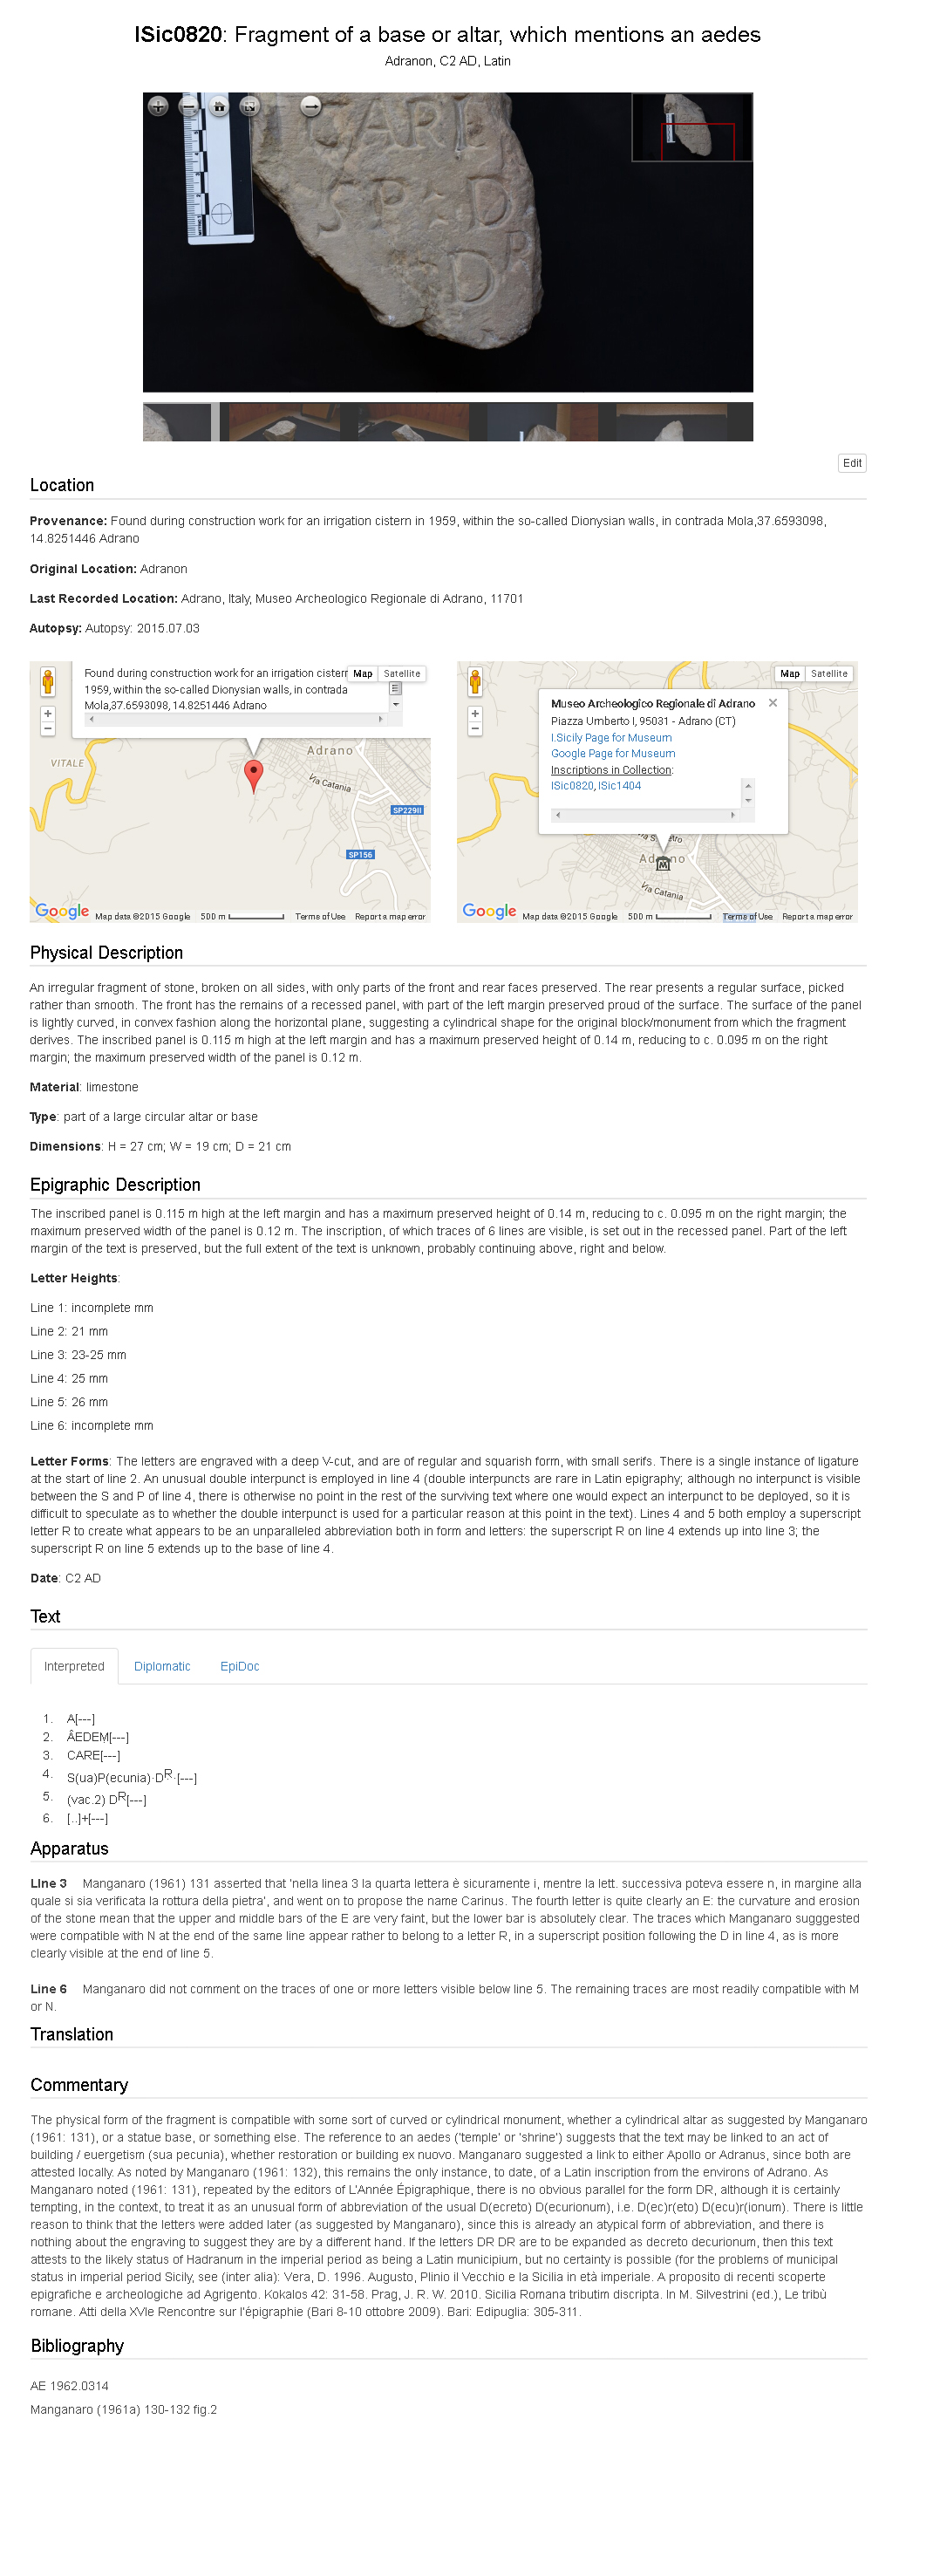
\includegraphics[width=0.6\columnwidth]{EAGLE2016ISicilyfinalcopy-img001.jpg}
\caption{sample edition}
\label{fig:1}
\end{figure}


\begin{figure}[!bp]
\centering
 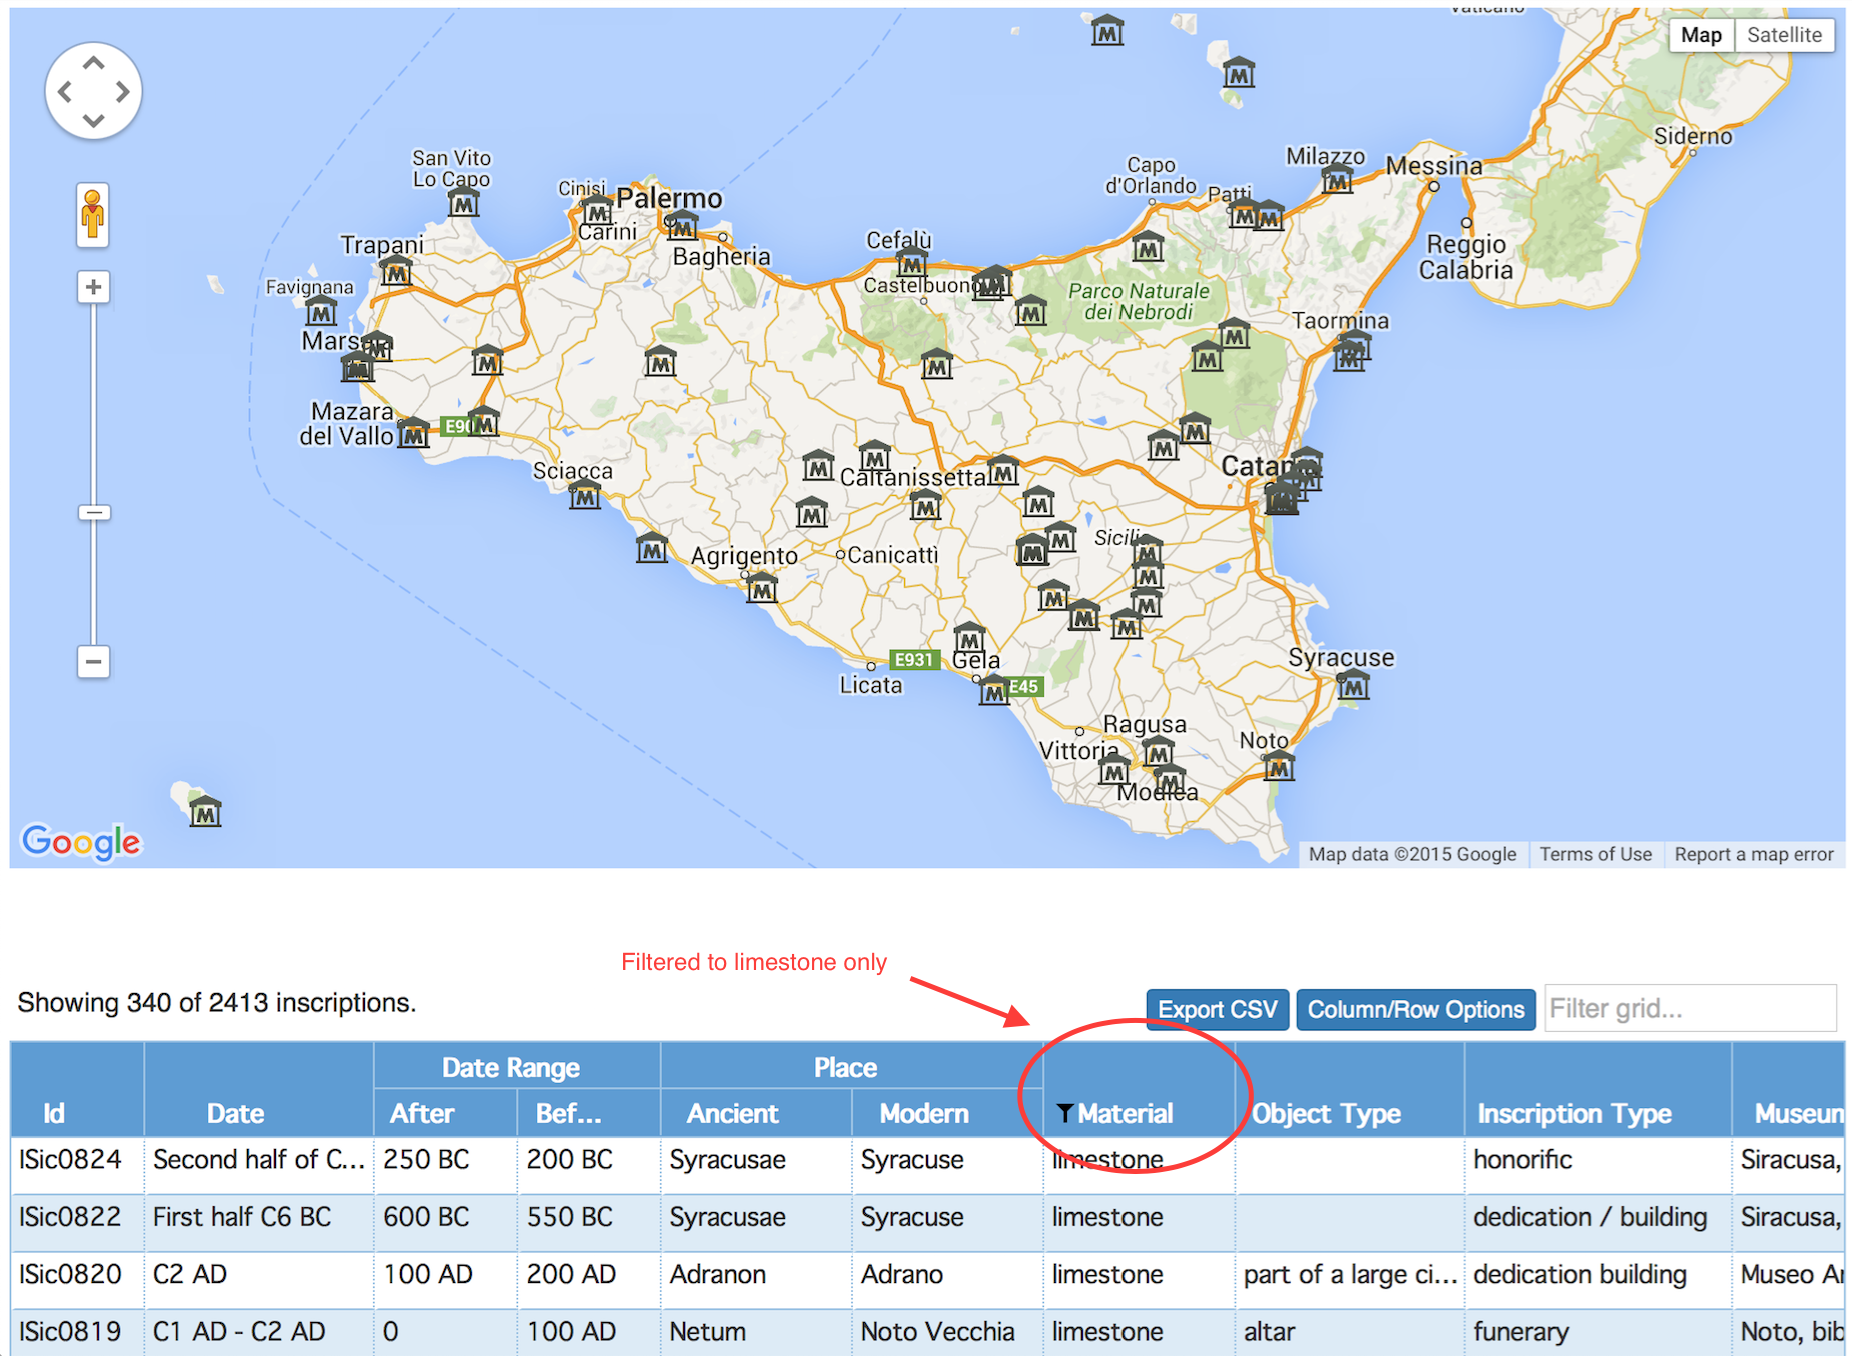
\includegraphics[width=\columnwidth]{EAGLE2016ISicilyfinalcopy-img002.png}
\caption{Screenshot of map-based searching (museum locations) and of part of the spreadsheet/grid search interface
employed in I.Sicily}
\label{fig:2}
\end{figure}
 



\section{Limitations and future ambitions}


The scale of the enterprise, and the available resources, mean that in its current form the project has limited itself
to inscriptions engraved on stone (the coverage of rupestral inscriptions/graffiti and of inscriptions painted on
stone/plaster is regrettably uneven). However, there is no reason in principle not to extend coverage in future to
include inscriptions on other materials. Similarly, although as noted above the current project does not include a
programme to mark up linguistic features of the texts, the commitment to the long-term maintenance of the corpus and
the open availability of the underlying XML records means that such a project would be entirely possible in the future.

A core principal of the project is that wherever possible an inscription record should be supported by recent autopsy
and not simply derived from the existing literature. Necessarily, this process is a slow one, and the majority of
records at this stage consist of information derived from secondary sources (earlier editions and other publications).
Individual inscription records will contain a clear indication of the editorial state of the record (from unchecked
through to fully edited) and additionally whether the record is underpinned by autopsy. In both cases, clear records
will be kept of editorial responsibility, autopsy and authorship as appropriate. In order to speed up the development
of the corpus, and to encourage those working on the material to take ownership of it for themselves, we aim to enable
individuals to submit new records and emendations or additions to existing records (such as translations, images,
location information), both in the Epigraphic database and the Museums database. To this end, we welcome collaboration
with those undertaking epigraphic projects in Sicily, and aim to offer the ability for other projects to publish their
editions through I.Sicily.\footnote{ We are currently establishing just such a collaboration with Prof.ssa M. Sgarlata
and Drs Lo Faro and Gradante, in support of their project to produce the volume of Inscriptiones Christianae Italiae
for the San Giovanni Catacombs in Siracusa.} We are also exploring the potential of the corpus as a teaching resource
both for epigraphy in general and for the teaching of EpiDoc. This latter aspect has already been initiated through a
Teaching Project Award (2014-2015) from the Humanities Division of the University of Oxford, and we aim to develop this
further in the coming year, as part of the work of incorporation and conversion of texts into the existing dataset.

It is our long-term ambition that I.Sicily might become the default location for the publication and dissemination of
Sicilian inscriptions; in the shorter term, we hope that it will serve as valuable portal in the world of Sicilian
epigraphy and of ancient world open linked data, greatly improving the accessibility of Sicilian epigraphy and so
enriching the study of the `crossroads of the Mediterranean’.




\section*{Acknowledgments}

I.Sicily gratefully acknowledges the financial support of the John Fell Fund of the
University of Oxford, and of the Warden and Scholars of the House or College of Scholars of Merton in the University of
Oxford.


\bibliographystyle{sapauth-eng}
\bibliography{../../EAGLE}

\end{document}
